%!TEX root = ../Thesis.tex

\chapter{Fahrspur-Bestimmung aus Trajektorie-Clustern}
\label{cha:lane_definition}

In diesem Kapitel wird beschrieben, wie aus den bereits identifizierten Trajektorie-Clustern
Geometrie-Informationen der Fahrspuren abgeleitet werden. Hierzu sind primär drei Schritte notwendig:
Bestimmung der Spur-Mittellinien, Bestimmung der Spurhüllen und anschließend die Partitionierung sich überlagernder
Spuren. Hinzu kommen weitere kleine Schritte, welche ebenfalls nachfolgend beschrieben werden.

\section{Ausfilterung von Spurwechselvorgängen}
\label{sec:real2_filter_lane_change}

Bevor mithilfe der im vorherigen Schritt gewonnenen Trajektorie-Cluster Mittellinien von Fahrspuren bestimmt
werden können, müssen diese nochmals vorverarbeitet werden. Die einzelnen Cluster enthalten teilweise
Bewegungsbahnen, welche Spurwechselvorgänge oder andere Abweichungen von einer Fahrspur beschreiben.
Diese Trajektorien müssen, so weit wie möglich,
entfernt werden, da sie die anschließende Geometrie-Bestimmung negativ beeinträchtigen. Die Trajektorien
eines Clusters sollten eindeutig einer realen Fahrspur zuzuordnen sein. In Abbildung
\ref{fig:real2_clusters_pre_postpro} sind beispielhaft zwei Cluster dargestellt, welche eine Vielzahl an
Spurwechselvorgängen enthalten.

\begin{figure}[H]
    \centering
    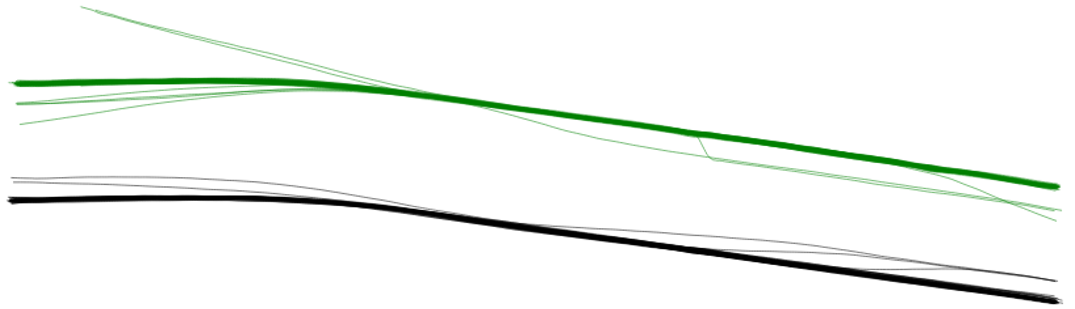
\includegraphics[width=0.8\linewidth]{../resources/img/umsetzung/U2/Clusters_Pre_Postprocessing}
    \caption{Trajektorie-Cluster mit Spurwechselvorgängen}
    \label{fig:real2_clusters_pre_postpro}
\end{figure}

Die Grundidee, welche der Ausfilterung der Abweichungen zugrunde liegt, ist, jene Trajektorien
aus einem Cluster zu entfernen, welche eine überdurchschnittlich hohe mittlere Distanz zu allen anderen
Trajektorien des Clusters besitzen. Als Distanzmaß wird erneut die LCSS Distanz verwendet.
Ein ähnlicher, Distanz-basierter Ausreißer-Detektionsansatz wird in \cite[]{Mirge2017} vorgestellt.
Der in dieser Arbeit verwendete Algorithmus ist in Listing \ref{lst:pseudo_post_processing} beschrieben.

\begin{lstlisting}[caption=Pseudocode Cluster Post-Processing, language=Pseudo, label=lst:pseudo_post_processing]
algorithm filterCluster:
  input:  unfiltered trajectories of cluster: trajsIn
  output: filtered trajectories of cluster

  meanTrajectoryDistances :=
    for each traj in trajsIn do
      yield mean LCSS distance of traj to all other trajectories of trajsIn
    end

  clusterCmpVal := select median of meanTrajectoryDistances as comparison value

  resultTrajs :=
    for each traj in trajsIn do
      if meanDist of traj < 1.5 * clusterCmpVal then
        yield trajs
      end
    end

  return resultTrajs
\end{lstlisting}

Das gewählte Verfahren ist einfach, eignet sich aber dennoch gut, um das gewünschte Ziel zu erreichen.
Die in Abbildung \ref{fig:real2_clusters_post_postpro} dargestellten Ergebnisse zeigen dies.
Aus den in Abbildung \ref{fig:real2_clusters_pre_postpro} enthaltenen Clustern wurden alle Trajektorien
mit Spurwechselvorgängen oder Abweichungen entfernt. Die Effektivität konnte auch durch die Anwendung
auf andere Datensätze bestätigt werden.
Wenn in einem Cluster viele Trajektorien Abweichungen von einer Spur besitzen, ist es möglich, dass der Algorithmus
diese nicht vollständig entfernt. Eine geringe Anzahl von Abweichungen beziehungsweise kleine Ausreißer
sind allerdings unproblematisch. 

\begin{figure}[H]
    \centering
    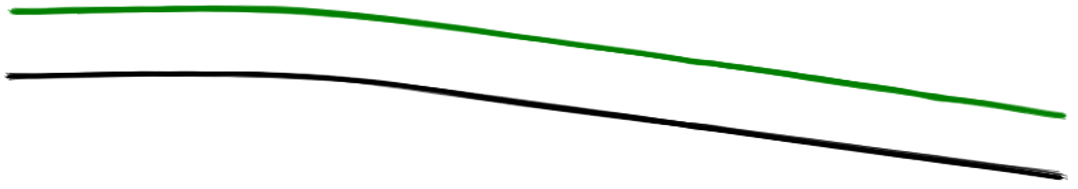
\includegraphics[width=0.8\linewidth]{../resources/img/umsetzung/U2/Clusters_Post_Postprocessing}
    \caption{Trajektorie-Cluster ohne Spurwechselvorgänge}
    \label{fig:real2_clusters_post_postpro}
\end{figure}

Zu beachten ist auch, dass die Zeitkomplexität des Verfahrens bei großen Trajektorie-Clustern
nicht unerheblich ist. Dies ist auf die Komplexität des LCSS Distanzmaßes zurückzuführen.
Bei der Untersuchung alternativer Vorgehensweise wurde allerdings klar, dass es grundlegend schwer ist,
dieses Problem performant zu lösen. In \cite[]{Meng2018} werden hierzu diverse Distanz- und Dichte-basierte
Arbeiten vorgestellt und verglichen. Da diese alle allerdings nicht weniger komplex sind und häufig
die verfolgten Ziele über die hier geforderten hinausgehen, wurde entschieden den oben beschriebenen Ansatz
beizubehalten. Durch die Parallelisierung der Berechnung der mittleren Abstände konnte die Performance
des Ansatzes außerdem nochmals deutlich gesteigert werden.

\section{Bestimmung Spurmittellinien}
\label{sec:real2_define_lane_centerline}

Nachdem die Trajektorie-Cluster nun weitestgehend von Fahrspurwechseln und anderen Abweichungen bereinigt
wurden, beschreiben die verbleibenden Bewegungsbahnen eines Clusters idealerweise eine Fahrspur.
Anhand dieser Trajektorien können daher nun die Mittellinie der Spuren bestimmt werden.

Die zu bestimmende Mittellinie verläuft durch die Mitte des entsprechenden
Trajektorie-Clusters. Die einzelnen Bewegungsbahnen besitzen jeweils leichte Abweichungen von dieser
\textit{``Ideallinie''}.
Als Spurmittellinie -- wie von \cite{Hu2005} vorgeschlagen -- jene Trajektorie zu wählen, welche die
kleinste Summe der Distanzen zu allen anderen Trajektorien eines Clusters besitzt, ist nicht praktikabel,
da die so gefunden Trajektorie nicht über ihre komplette Länge in der Mitte des Clusters verlaufen muss.
Auf eine Bestimmung der Mittellinie mittels linearer oder polynomialer Regression, wie beispielsweise in
\cite[]{Chen2014} oder \cite[]{Melo2006},
wurde ebenfalls verzichtet. Der Grund hierfür ist, dass einerseits die Komplexität der Fahrbahnverläufe
nicht bekannt ist und andererseits das Erlernen der Spurrepräsentation zu aufwendig ist.

Der in dieser Arbeit gewählte Ansatz zur Bestimmung der Spurmittellinien macht sich die von Atev et al.
vorgestellte Notation einer relativen Position innerhalb einer Trajektorie zu nutze, welche in
Gleichung \ref{eq_atev_relPos} und \ref{eq_atev_findPointAtRelPow} gegeben ist.
Die Koordinaten der Spurlinien ergeben sich aus den Mittelwerten von Trajektorie-Punkten, welche sich
alle an der selben relativen Position befinden. Der verwendete Algorithmus ist nachfolgend beschrieben.
\begin{lstlisting}[caption=Pseudocode Cluster Post-Processing, language=Pseudo, label=lst:pseudo_post_processing]
algorithm calculateCenterline:
  input:  trajectories of cluster: trajsIn
  output: centerline of lane

  meanTrajLength := calculate mean point length of trajectories
  relPositions := define range with relative positions of size meanTrajLength
                  and step-size (1 / meanTrajLength)

  centerline :=
    for each relP in relPositions do
      pointsAtRelPos := get points at relP for each traj in trajsIn
      yield mean of all points in pointsAtRelPos
    end

  return centerline
\end{lstlisting}

Da die Form und der Verlauf von Trajektorien eines Clusters sich nur wenig unterscheiden, liefert dieses
Vorgehen gute Ergebnisse. In Abbildung \ref{fig:real2_results_centerline_detection} a) ist beispielhaft
dargestellt, wie eine Mittellinien innerhalb eines Trajektorie-Clusters verlaufen.
In \ref{fig:real2_results_centerline_detection} b) sind alle Spurmittellinien der Neckartor-Kreuzung,
welche auf die oben beschriebene Weise bestimmt wurden, abgebildet.

% TODO: Bild mit Spurmittellinien in Aufnahme
\begin{figure}[H]
    \centering
    \subfloat[]{{
        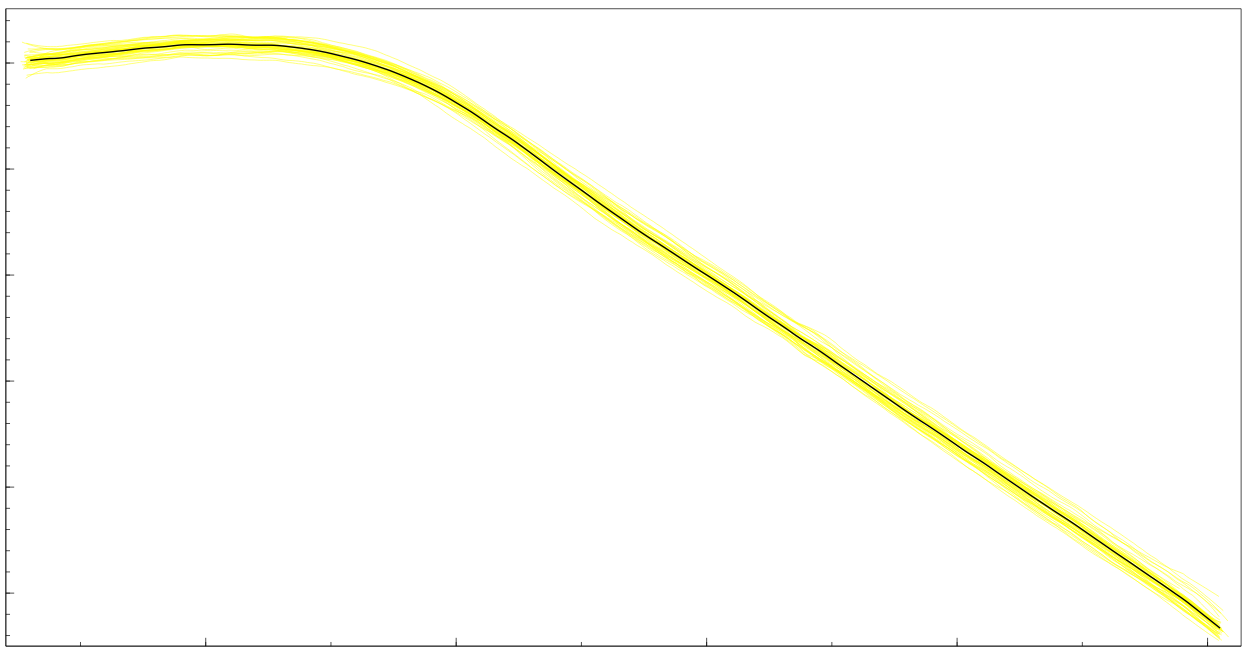
\includegraphics[align=c, width=0.45\linewidth]{../resources/img/umsetzung/U2/cluster_with_centerline}
    }}
    \qquad
    \subfloat[]{{
        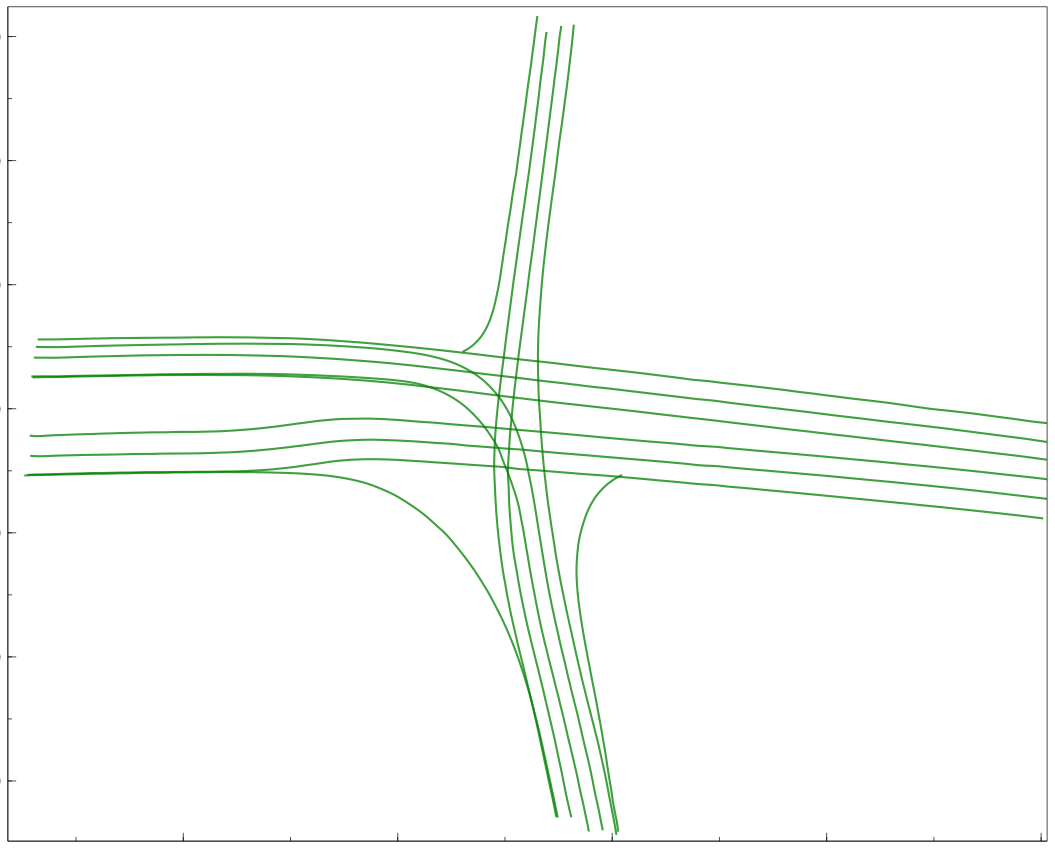
\includegraphics[align=c, width=0.4\linewidth]{../resources/img/umsetzung/U2/laneCenters}
    }}
    \caption{Spurmittellinie in einem Trajektoriecluster a), Spurmittellinien Neckartor-Kreuzung b)}
    \label{fig:real2_results_centerline_detection}
\end{figure}

\section{Bestimmung Spurhüllen}
\label{sec:real2_define_lane_envelope}

% Erklärung SpurDefinition (LaneEstimate) Über Nodes? Siehe Rel. Work.
% Bestimmung benachbarter Spuren
% Bestimmung paralleler Spuren
% Bestimmung des mittleren Abstands zwischen zwei parallelen Spurpaaren
% Bestimmung Envelope-Punkte


\section{Partitionierung von Fahrspuren}
\label{sec:real2_lane_partitioning}

% Arbeiten nur noch mit LaneEstimates
% Grundidee: Sich überschneidende Spuren an Schnittpunkte partitionieren
% Problem: welche Spur ganz lassen und welche partitionieren
% Aufteilung in drei Spur-Typen (isolated, primary, secundary)
% Finden von sich überlappenden Spurpaaren
% Entscheidung für zu partitionierende Spuren (nach Kriterien)
% Partitionierung